\clearpage
\subsection{Direct measurement of the cumulative change}
\label{sec:cumulative-speedup}
The preceding sections compare successive changes on different target sets.
To measure the cumulative change directly, we now run the original baseline
and final deployed calculation on identical integrals. We retain the
coupled vacuum family of Eq.~\eqref{eq:coupled-vacuum}, with unit massless
powers, two to four distinct massive denominators and fixed positive
integer mass ratios. We set the common squared-mass scale to \(\mu=1\),
as in the preceding comparisons. Each target has the same prescribed master basis
in every comparison.

The first control uses the saved original Kira 3.1 executable, whose file
hash agrees with the first frozen cost comparison. It generates the full
Euler and mass partial-fraction equation pool and reduces each mass
profile separately at every requested loop order. The Euler seeds extend
through the largest target power, and the mass-pair identities extend
through one additional power. A second control uses exactly the same
requests, equation generation, reader and verification, with the later
project executable used in Section~\ref{sec:higher-loop-acceleration}.
Its learned policies are disabled. Comparing these controls separates
the executable change from the subsequent removal of repeated reductions.

The final route remains the validation-selected implementation from
Section~\ref{sec:exact-backend}. It evaluates the selected recurrences directly and calls Kira only if
the exact check fails. It uses the fixed extreme-power recurrence,
shares coefficients in \(z=L(d-2)\), checks them through the independent
Taylor construction, expands them with compiled exact arithmetic and
saves lossless binary output. It retains the existing Kira fallback.
No model is retrained and no strategy is selected from the cumulative
test results. These calculations use explicitly supplied identities;
the test does not invoke native generation of a general multiloop IBP
system.

We declare eight new groups of three mass profiles, one each with
\(R=2,3,4\), and request every loop order \(L=1,\ldots,12\).
Two groups use each maximum total massive power \(8,10,12,14\).
The requested target counts per profile are \(16,32,48,64\), respectively,
capped by the available index vectors. The mass profiles are new, while
index shapes can overlap earlier data within this restricted family.
A separate upper-bound pilot checks executable compatibility and
resource use. We then freeze the implementations, executable hashes,
final deployment choice and all reserved requests.

Five repetitions of each method give 120 complete workflows.
Both controls use the same scheduler-provided job-local scratch.
Four allocated CPU slots process independent groups on one scheduled
node. Each worker binds to a distinct available physical core, and
every matched comparison remains bound to that core,
with a shuffled sequential order within each three-method block. Each trial starts a fresh
worker process and uses ordinary filesystem caching. Content-addressed
storage can reuse an identical saved output on a repeated trial in any
arm, while each arm recomputes its reduction. The primary time includes
process startup, input loading, equation construction, exact algebra,
verification, output saving, and reading and decoding the full output.
It also includes the diagnostic evidence written inside each worker.
Queue waiting, offline training and the later independent audit lie
outside this time. We separately retain calculation times before
final output saving and reading.

Let \(T_{abr}\) denote the primary time for method \(a\), batch \(b\)
and repetition \(r\). We compare the medians within each batch and
combine the eight ratios through
\begin{equation}
 \widetilde T_{ab}=\operatorname{median}_{r=1,\ldots,5}T_{abr},
 \qquad
 R_T=\exp\!\left[\frac{1}{8}\sum_{b=1}^{8}
 \log\frac{\widetilde T_{\mathrm{final},b}}
               {\widetilde T_{\mathrm{original},b}}\right],
 \qquad
 S=\frac{1}{R_T}.
 \label{eq:cumulative-ratio}
\end{equation}
Here \(R_T\) is the final-to-original time ratio and \(S\) is the cumulative
speedup. The percentage of time saved is \(100(1-R_T)\).
A descriptive 95\% interval resamples the eight complete batches
10,000 times, keeping all repetitions and methods within each batch.
This direct comparison uses neither products of earlier ratios nor
different input sets for the two methods.

The measured time ratio is 0.001839, with descriptive interval
\([0.001653,0.002049]\). It corresponds to 543.815 times faster execution,
with interval \([488.134,605.064]\), and 99.82\% less time.
The ratio to the later full-pool control is 0.012,
corresponding to 81.170 times faster execution.
The calculation subtotal excludes outer worker startup and final output
saving and reading, while retaining every Kira startup within the
baseline reduction. Its final-to-original ratio is 0.000294,
or 3402.846 times faster.
Summing one primary-time median per batch gives 1027.781 seconds
for the original control and 1.922 seconds for the final route,
a workload speedup of 534.881. This sum weights large batches
by their elapsed time, whereas Eq.~\eqref{eq:cumulative-ratio} gives
equal weight to each batch. Figure~\ref{fig:cumulative-speedup} shows
the absolute times and individual speedups.

Within each batch, every method and repetition returns the same exact
expanded coefficients. All 120 reserved workflows complete with no
failure or fallback. Each baseline arm makes 1,440 Kira calls;
the final arm makes none on these successful requests. The independent
audit checks 27960 nonzero target--master coefficient polynomials
after substituting each loop order, using the earlier loop-dependent
Taylor formula. It also regenerates all
288 distinct baseline systems, checks their input hashes and
uses SymPy to read 1464 coefficient positions directly from
saved Kira exports. The two baseline executables receive identical
systems at each mass profile and loop order. The maximum sampled
worker process-tree memory is 78.488 MiB and temporary solver storage
is 1.238 MiB.

The cumulative saving includes shared symbolic reductions, direct
checked recurrences, compiled expansion and reduced output costs.
The fixed-rule deployment makes this a measurement of the complete
mathematical and implementation change. It supplies no separate
ML-only speedup estimate. General scattering families and native
generation of broader high-loop IBP systems remain outside this
comparison. The frozen inputs, implementations, individual timings,
raw exports and audits accompany the report~\cite{KiraCumulativeData}.

\begin{figure}[htbp]
 \centering
 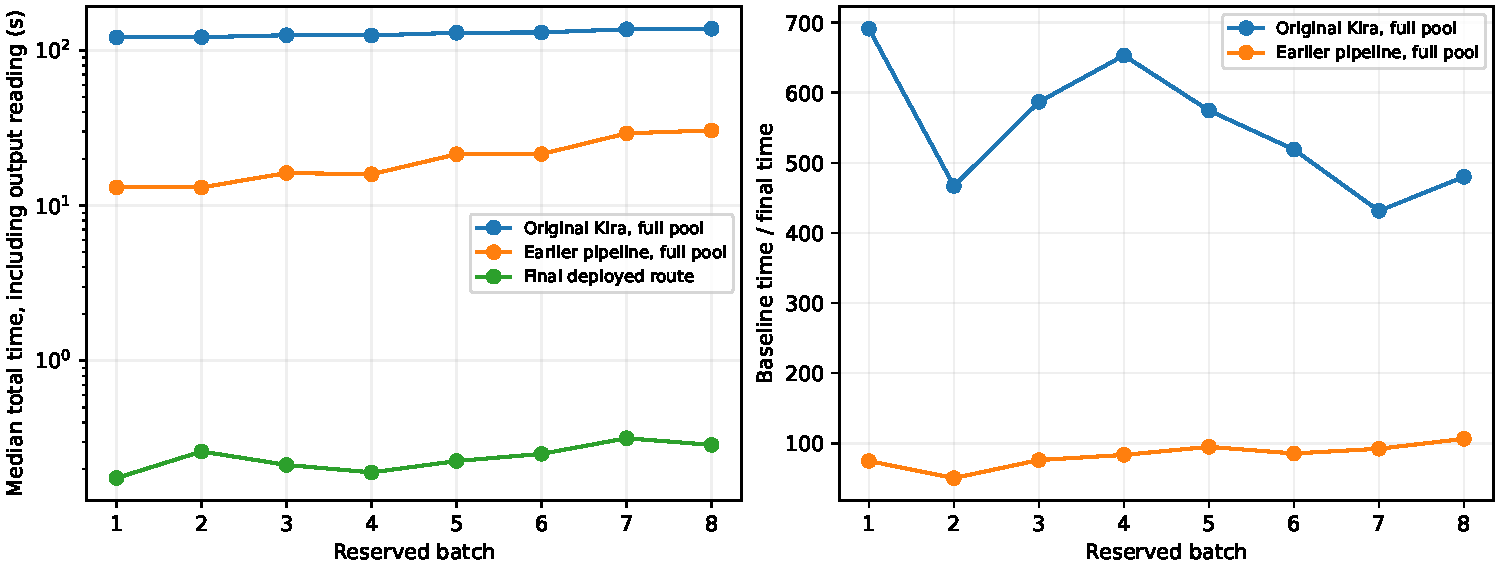
\includegraphics[width=\textwidth]{figures/cumulative_speedup.pdf}
 \caption{Direct cumulative comparison on identical reserved vacuum
 batches. The left panel shows median total times, including output
 reading, on a logarithmic scale. The right panel divides each
 baseline median by the final-route median. Each point uses five
 repetitions, three mass profiles and loop orders one through twelve.}
 \label{fig:cumulative-speedup}
\end{figure}
